\documentclass[aspectratio=169]{beamer}

% Lines related with beamer theme
\usetheme[progressbar=frametitle]{metropolis}
%\setbeamertemplate{frame numbering}[fraction]

\setbeamertemplate{caption}{\raggedright\insertcaption\par}


% Lines related with latex packages
\usepackage{amsmath,amsfonts,amssymb}
\usepackage{mathtools} 
\usepackage{multicol}
\usepackage{threeparttable}
\usepackage{booktabs, makecell}
\usepackage{multirow}
\usepackage{tikz}
\usetikzlibrary{arrows.meta,positioning,fit}
\usepackage{xcolor}
\usepackage{bm}
\usepackage{adjustbox}
\usepackage{graphicx}
\usepackage{pdfpages} 
\usepackage{makecell}


% First slide info
\author{Antón de la Fuente Suárez-Pumariega}
\title{Decentralized decision power and information sharing in horizontal logistics collaboration}
\institute{
\includegraphics[scale=0.08]{maastricht-logo}}
\date{\today}
\def\titlepage{
  \usebeamertemplate{title page}
}

\begin{document}

% I few lines selecting some parameters of the beamer theme
\metroset{block=fill}
\metroset{sectionpage=progressbar}
\metroset{subsectionpage=progressbar}

%Tittle slide
\maketitle

%Table of contents
\begin{frame}{Agenda}
\setbeamertemplate{section in toc}[sections numbered]
	\tableofcontents
\end{frame}

%\metroset{sectionpage=none}
\section{Introduction}

\begin{frame}{Horizontal logistics collaboration}

\begin{itemize}
\setlength\itemsep{1em}
\item<1-> Cooperation between agents at the same level in the supply chain.
\item<2-> Two main branches:
\medskip

\begin{itemize}
\setlength\itemsep{1em}
\item<2-> Centralized $\rightarrow$ Central planning.
\item<2-> Decentralized $\begin{cases}
\text{Auction-based.}\\[5pt]
\text{\alert<3>{Non auction-based.}}
\end{cases}$
\end{itemize}
\end{itemize}

\usetikzlibrary{arrows.meta,positioning}
\end{frame}

\section{The network design - multicommodity flow problem}

%\begin{frame}{\secname}
%
%\begin{columns}
%\begin{column}{0.5\textwidth}
%\vspace{1cm}
%
%\textbf{Commodities:}
%\vspace{-0.5cm}
%\begin{table}
%\begin{tabular}{ccccc}
%& Origin & Terminal & Size & Revenue \\\hline
%$\color{red}k^1$ & 1 & 2 & 1 & 10 \\
%$\color{red}k^2$ & 1 & 4 & 1 & 10 \\
%$\color{red}k^3$ & 3 & 1 & 1 & 10 
%\end{tabular}
%\end{table}
%\bigskip
%
%\textbf{Edges:}
%\vspace{-0.5cm}
%\begin{table}
%\begin{tabular}{ccc}
%& Capacity & \makecell{Activation \\ cost} \\\hline
%$\forall$ edge & 2 & 5 \\
%\end{tabular}
%\end{table}
%\end{column}
%
%\begin{column}{0.5\textwidth}
%\only<1>{
%\begin{figure}
%	\centering	
%	\begin{tikzpicture}
%	\begin{scope}[every node/.style={circle,draw,align=center,text width = 5pt}]
%		\node (1) at (0,0) {1};
%		\node (2) at (3,0) {2};
%		\node (3) at (0,-3) {3};
%		\node (4) at (3,-3) {4};
%	\end{scope}
%	\begin{scope}[every edge/.style={dashed,draw,bend left=10}]
%		\draw[-stealth] (1) edge node[above] {\phantom{$k^1$}} (2);
%		\draw[-stealth] (2) edge (1);
%		\draw[-stealth] (1) edge (3);
%		\draw[-stealth] (3) edge node[left] {\phantom{$k^3$}} (1);
%		\draw[-stealth] (1) edge node[right=9pt] {\phantom{$k^2$}} (4);
%		\draw[-stealth] (4) edge (1);
%		\draw[-stealth] (2) edge (3);
%		\draw[-stealth] (3) edge (2);
%		\draw[-stealth] (2) edge (4);
%		\draw[-stealth] (4) edge (2);
%		\draw[-stealth] (3) edge (4);
%		\draw[-stealth] (4) edge (3);
%	\end{scope}
%	\end{tikzpicture}
%	\caption{Original network.}
%	\end{figure}
%}
%
%\only<2>{
%\begin{figure}
%	\centering	
%	\begin{tikzpicture}
%	\begin{scope}[every node/.style={circle,draw,align=center,text width = 5pt}]
%		\node (1) at (0,0) {1};
%		\node (2) at (3,0) {2};
%		\node (3) at (0,-3) {3};
%		\node (4) at (3,-3) {4};
%	\end{scope}
%	\begin{scope}[every edge/.style={draw,bend left=10}]
%		\draw[-stealth,red] (1) edge node[above] {\phantom{$k^1$}}(2);
%	
%		\draw[-stealth,red] (3) edge node[left] {\phantom{$k^3$}} (1);
%		\draw[-stealth,red] (1) edge node[right=9pt] {\phantom{$k^2$}} (4);
%	
%	\end{scope}Example
%	\end{tikzpicture}
%	\caption{Design of the network.}
%	\end{figure}
%}
%
%\only<3>{
%\begin{figure}
%	\centering	
%	\begin{tikzpicture}
%	\begin{scope}[every node/.style={circle,draw,align=center,text width = 5pt}]
%		\node (1) at (0,0) {1};
%		\node (2) at (3,0) {2};
%		\node (3) at (0,-3) {3};
%		\node (4) at (3,-3) {4};
%	\end{scope}
%	\begin{scope}[every edge/.style={draw,bend left=10}]
%		\draw[-stealth,red] (1) edge node[above] {$k^1$} (2);
%		\draw[-stealth,red] (3) edge node[left] {$k^3$} (1);
%		\draw[-stealth,red] (1) edge node[right=9pt] {$k^2$} (4);
%		
%	\end{scope}
%	\end{tikzpicture}
%	\caption{Route the commodities.}
%	\end{figure}
%}
%\end{column}
%
%\end{columns}
%\end{frame}

%\begin{frame}{\secname: ILP}
%\begin{itemize}
%\item We model the problem as an ILP, $\quad \pmb{P_i}\ \forall i \in N$.
%
%\begin{align}
%        &  P_i: \quad \max  &  \sum_{k\in \Theta^i} \sum_{e \in \delta^+(t(k))\cap E^i} f_e^k \cdot d_k \cdot r_k - \sum_{e\in E^i} u_e\cdot c_e \hspace{20pt} &&
%	\end{align}
%	
%\item Subject to different constraints
%\end{itemize}
%\end{frame}

\begin{frame}{\secname}

\begin{columns}

\begin{column}{0.5\textwidth}
\vspace{1cm}

\textbf{Commodities:}
\vspace{-0.5cm}
\begin{table}
\begin{tabular}{ccccc}
& Origin & Terminal & Size & Revenue \\\hline
$\color{red}k^1$ & 1 & 2 & 1 & 10 \\
$\color{red}k^2$ & 1 & 4 & 1 & 10 \\
$\color{red}k^3$ & 3 & 1 & 1 & 10 \\
$\color{blue}k^4$ & 2 & 4 & 1 & 10
\end{tabular}
\end{table}
\bigskip

\textbf{Edges:}
\vspace{-0.5cm}
\begin{table}
\begin{tabular}{ccc}
& Capacity & \makecell{Activation \\ cost} \\\hline
$\forall$ edge & 2 & 5 \\
\end{tabular}
\end{table}
\end{column}

\begin{column}{0.5\textwidth}
\only<1>{
\begin{figure}
	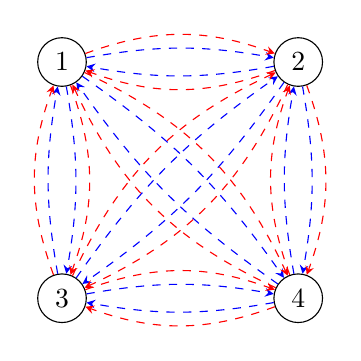
\begin{tikzpicture}
	\centering	
	\begin{scope}[every node/.style={circle,draw,align=center,text width = 5pt}]
		\node (1) at (0,0) {1};
		\node (2) at (3,0) {2};
		\node (3) at (0,-3) {3};
		\node (4) at (3,-3) {4};
	\end{scope}
	\begin{scope}[every edge/.style={dashed,draw,bend left=10},blue]
		\draw[-stealth] (1) edge (2);
		\draw[-stealth] (2) edge (1);
		\draw[-stealth] (1) edge (3);
		\draw[-stealth] (3) edge (1);
		\draw[-stealth] (1) edge (4);
		\draw[-stealth] (4) edge (1);
		\draw[-stealth] (2) edge (3);
		\draw[-stealth] (3) edge (2);
		\draw[-stealth] (2) edge (4);
		\draw[-stealth] (4) edge (2);
		\draw[-stealth] (3) edge (4);
		\draw[-stealth] (4) edge (3);
		
	\end{scope}
	\begin{scope}[every edge/.style={dashed,draw,bend left=20},red]
		\draw[-stealth] (1) edge (2);
		\draw[-stealth] (2) edge (1);
		\draw[-stealth] (1) edge (3);
		\draw[-stealth] (3) edge (1);
		\draw[-stealth] (1) edge (4);
		\draw[-stealth] (4) edge (1);
		\draw[-stealth] (2) edge (3);
		\draw[-stealth] (3) edge (2);
		\draw[-stealth] (2) edge (4);
		\draw[-stealth] (4) edge (2);
		\draw[-stealth] (3) edge (4);
		\draw[-stealth] (4) edge (3);
	\end{scope}
	\end{tikzpicture}
	\caption{Original network.}
	\end{figure}
}

\only<2>{
\begin{figure}
	\centering	
	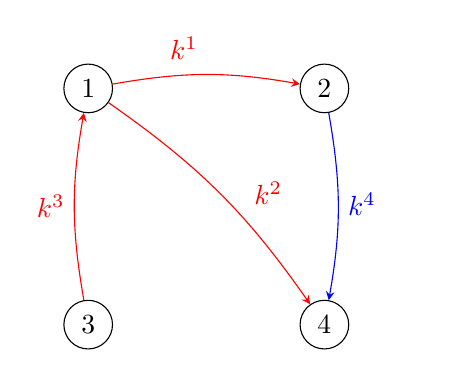
\begin{tikzpicture}
	\begin{scope}[every node/.style={circle,draw,align=center,text width = 5pt}]
		\node (1) at (0,0) {1};
		\node (2) at (3,0) {2};
		\node (3) at (0,-3) {3};
		\node (4) at (3,-3) {4};
	\end{scope}
	\begin{scope}[every edge/.style={draw,bend left=10}]
		\draw[-stealth,red] (1) edge node[above] {$k^1$\phantom{, $\color{red}k^2$}}(2);
		\draw[-stealth,red] (3) edge node[left] {$k^3$} (1);
		\draw[-stealth,red] (1) edge node[right=9pt] {$k^2$} (4);
		\draw[-stealth,blue,bend left=20] (2) edge  node[right] {$k^4$\phantom{, $\color{red}k^2$}} (4);
	\end{scope}
	\end{tikzpicture}
	\caption{Solution without cooperation.}
	\end{figure}
}

\only<3>{
\begin{figure}
	\centering	
	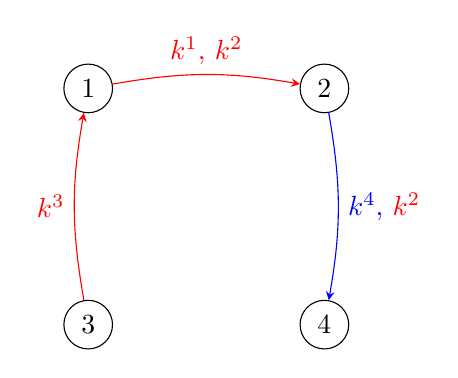
\begin{tikzpicture}
	\begin{scope}[every node/.style={circle,draw,align=center,text width = 5pt}]
		\node (1) at (0,0) {1};
		\node (2) at (3,0) {2};
		\node (3) at (0,-3) {3};
		\node (4) at (3,-3) {4};
	\end{scope}
	\begin{scope}[every edge/.style={draw,bend left=10}]
		\draw[-stealth,red] (1) edge node[above] {$k^1$, $k^2$}(2);
		\draw[-stealth,red] (3) edge node[left] {$k^3$} (1);
		\draw[-stealth,blue,bend left=20] (2) edge  node[right] {$k^4$, $\color{red}k^2$} (4);
	\end{scope}
	\end{tikzpicture}
	\caption{Cooperative solution.}
	\end{figure}
}
\end{column}

\end{columns}
\end{frame}

\section{Allocation rule}

\begin{frame}{\secname}
\begin{enumerate}
	\setlength\itemsep{1em}
    \item The revenues generated by any served commodity are
    allocated to its owner.
    \item The activation cost of any active edge is paid by its owner.
    \item The price of using an unit of capacity on an edge $e\in E$ owned by agent $w(e)$ for any other member of the coalition, $i\in N\setminus\{w(e)\}$, is equal to $\dfrac{c_e}{q_e}$.
\end{enumerate}
\end{frame}


\section{Three systems with central authority}
\begin{frame}{\secname}
\begin{itemize}
\setlength\itemsep{1em}

\item A central authority with certain decision power.
\item Agents have to share certain amount of information to cooperate.
\item 3 systems: $\begin{cases}
\text{Fully centralized cooperation system (FCCS),}\\
\text{Partial cooperation system (PCS),} \\
\text{Residual cooperation system (RCS).}
\end{cases}$
\end{itemize}
\end{frame}

\subsection*{Fully centralized cooperative system (FCCS)} 
\begin{frame}{\subsecname}
\begin{itemize}
\setlength\itemsep{1em}
\item A central planning system $\Longrightarrow$ Central authority with \alert{full information} and \alert{all the decision power.}
\item Commodities and edges of all the agents are aggregated into a single bigger problem.
\item Final profit allocation must be \alert{individually rational}.
\end{itemize}
\end{frame}

\subsection*{Partial cooperative system (PCS)}

%\begin{frame}{\subsecname}
%Agents solve the network design - problem in two stages:
%\begin{enumerate}
%	\setlength\itemsep{1em}
%	\item Agents decide which edges to activate
%	\item The central authority routes the commodities %through the active edges
%\end{enumerate}
%\end{frame}

%\begin{frame}{\subsecname}
%
%\begin{figure}[ht!]
%\centering
%\begin{adjustbox}{width=\textwidth, totalheight=\textheight-2\baselineskip,keepaspectratio}
%\begin{tikzpicture}
%	\begin{scope}[every node/.style={rectangle,draw,thick,minimum height=16pt,minimum width =30pt}]
%		\node (A1) at (-4,0) {Agent 1 solves $P_1$};
%		\node[right =10pt of A1] (A2) {Agent 2 solves $P_2$};
%		\node[draw=none,right =10pt of A2] (pass) {$\cdots$ };
%		\node[right =10pt of pass] (An) {Agent $n$ solves $P_n$};
%		\node[align = left,text width=7cm] (shares) at (0,-2.5) {Agents share with  the  central planner:
%		\begin{itemize}
%			\itemsep-3pt 
%        		\item No-cooperation payoff, $P^*_i\  \forall i \in N$.
%        		\item The edges they activate.
%        		\item All their commodities.
%   		 \end{itemize}
%    };
%    \node[below = of shares,align = center,text width=6cm] (central) {Central planner routes all the commodities through the edges the agents have activated.};
%    
%    \node [fit=(A1) (An) (shares),draw,dashed,thick,blue] {};
%    \node[draw=none,blue] (Stage1) at (-6.8,-1.8) {Stage 1}	;
% 	\node [fit=(central) ,draw,dashed,thick,red] {};
% 	\node[draw=none,red] (Stage2) at (-4.3,-5.5) {Stage 2}	;
%	
%	\end{scope}
%	
%	\begin{scope}
%	\draw[-{Latex[length=2mm]}] (A1.south) |- (shares.west);
%	\draw[-{Latex[length=2mm]}] (A2) edge (A2.south|-shares.north);
%	\draw[-{Latex[length=2mm]}] (An.south) |- (shares.east);
%	\draw[-{Latex[length=2mm]}] (shares) edge (central);
%
%	\end{scope}
%\end{tikzpicture}
%\end{adjustbox}
%\end{figure}
%\end{frame}


\begin{frame}{\subsecname}
\begin{figure}[ht!]
\centering
\begin{adjustbox}{width=\textwidth, totalheight=\textheight-2\baselineskip,keepaspectratio}
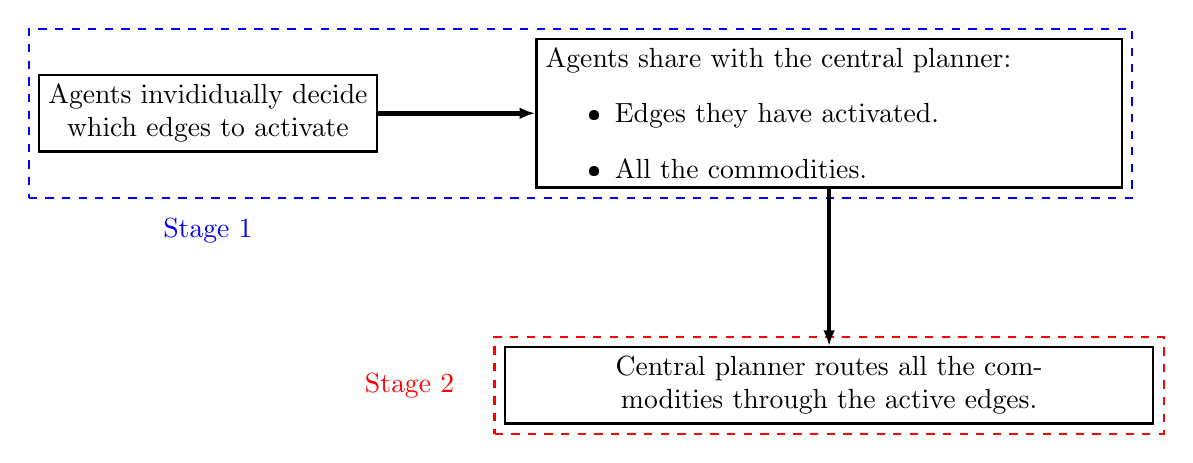
\begin{tikzpicture}
	\begin{scope}[every node/.style={rectangle,draw,thick,minimum height=16pt,minimum width =30pt}]
		\node[align = center] (A) at (-4,0) {Agents invididually decide \\ which edges to activate};
		\node[right =2cm of A,align = left,text width=7.2cm] (B) {Agents share with  the  central planner:
		\begin{itemize}

        		\item Edges they have activated.
        		\item All the commodities.
   		 \end{itemize}
    };
    		\node[below =2cm of B,align = center,text width=8cm] (C) {Central planner routes all the commodities through the active edges.};
    		
    
	 \node [fit=(A) (B),draw,dashed,thick,blue] {};
     \node[below =0.7cm of A,draw=none,blue] (Stage1) {Stage 1}	;
 	 \node [fit=(C) ,draw,dashed,thick,red] {};
 	 \node[left =0.5cm of C,draw=none,red] (Stage2) {Stage 2}	;    
 
	\end{scope}
	
	\begin{scope}
	\draw[-{Latex[length=2mm]},line width=1.7pt] (A) edge (B);
	\draw[-{Latex[length=2mm]},line width=1.7pt] (B) edge (C);

	\end{scope}
	\end{tikzpicture}
\end{adjustbox}
\end{figure}
\end{frame}

\subsection*{Residual cooperation system (RCS)}

%\begin{frame}{\subsecname}
%\begin{figure}[ht!]
%\centering
%\begin{adjustbox}{width=\textwidth, totalheight=\textheight-2\baselineskip,keepaspectratio}
%\begin{tikzpicture}
%	\begin{scope}[every node/.style={rectangle,draw,thick,minimum height=16pt,minimum width =30pt}]
%		\node (A1) at (-4,0) {Agent 1 solves $P_1$};
%		\node[right =10pt of A1] (A2) {Agent 2 solves $P_2$};
%		\node[draw=none,right =10pt of A2] (pass) {$\cdots$ };
%		\node[right =10pt of pass] (An) {Agent $n$ solves $P_n$};
%		\node[below = of A1,align = center] (A1impl) {Agent 1 \\ implements $P_1^*$};
%		\node[below = of A2,align = center] (A2impl) {Agent 2 \\ implements $P_2^*$};
%		\node[draw=none,below =35pt of pass] (pass2) {$\cdots$ };
%		\node[below = of An,align = center] (Animpl) {Agent n \\ implements $P_n^*$};
%		\node[align = left,text width=7.2cm] (shares) at (0,-4.5){Agents share with  the  central planner:
%		\begin{itemize}
%
%        		\item Edges with residual capacity.
%        		\item Residual commodities.
%   		 \end{itemize}
%    };
%    \node[below = of shares,align = center,text width=8cm] (central) {Central planner routes the residual commodities through the edges with residual capacity.};
%    
%	  \node [fit=(A1) (An) (shares),draw,dashed,thick,blue] {};
%    \node[draw=none,blue] (Stage1) at (-6.7,-3) {Stage 1}	;
% 	\node [fit=(central) ,draw,dashed,thick,red] {};
% 	\node[draw=none,red] (Stage2) at (-5.3,-7) {Stage 2}	;    
%    
%	\end{scope}
%	
%	\begin{scope}
%	\draw[-{Latex[length=2mm]}] (A1) edge (A1impl);
%	\draw[-{Latex[length=2mm]}] (A2) edge (A2impl);
%	\draw[-{Latex[length=2mm]}] (An) edge (Animpl);
%	\draw[-{Latex[length=2mm]}] (A1impl.south) |- (shares.west);
%	\draw[-{Latex[length=2mm]}] (A2impl) edge (A2.south|-shares.north);
%	\draw[-{Latex[length=2mm]}] (Animpl.south) |- (shares.east);
%	\draw[-{Latex[length=2mm]}] (shares) edge (central);
%
%	\end{scope}
%\end{tikzpicture}
%\end{adjustbox}
%\end{figure}
%\end{frame}


\begin{frame}{\subsecname}
\begin{figure}[ht!]
\centering
\begin{adjustbox}{width=\textwidth, totalheight=\textheight-2\baselineskip,keepaspectratio}
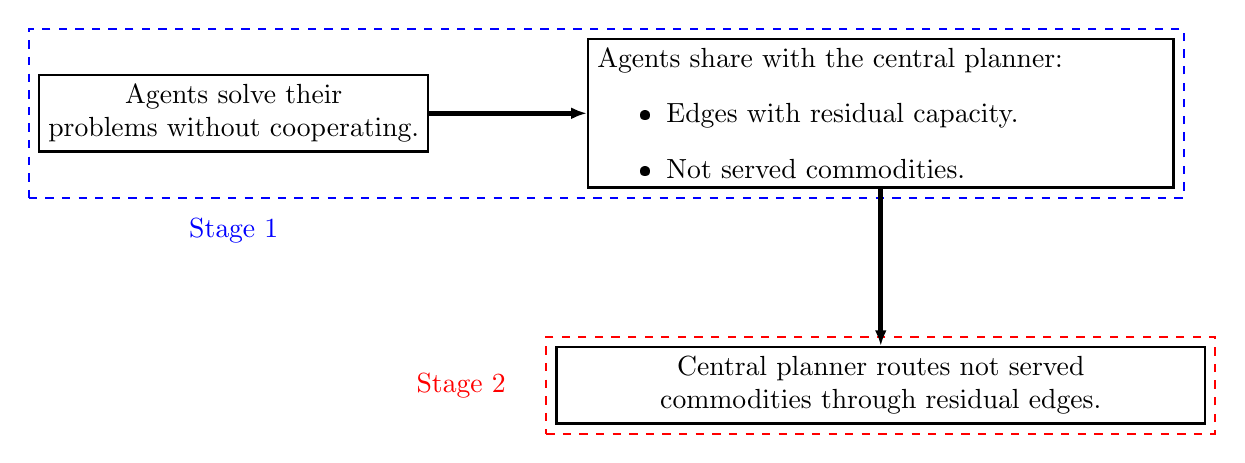
\begin{tikzpicture}
	\begin{scope}[every node/.style={rectangle,draw,thick,minimum height=16pt,minimum width =30pt}]
		\node[align = center] (A) at (-4,0) {Agents solve their\\ problems  without cooperating.};
		\node[right =2cm of A,align = left,text width=7.2cm] (B) {Agents share with  the  central planner:
		\begin{itemize}

        		\item Edges with residual capacity.
        		\item Not served commodities.
   		 \end{itemize}
    };
    		\node[below =2cm of B,align = center,text width=8cm] (C) {Central planner routes not served commodities through residual edges.};
    		
    
	 \node [fit=(A) (B),draw,dashed,thick,blue] {};
     \node[below =0.7cm of A,draw=none,blue] (Stage1) {Stage 1}	;
 	 \node [fit=(C) ,draw,dashed,thick,red] {};
 	 \node[left =0.5cm of C,draw=none,red] (Stage2) {Stage 2}	;    
 
	\end{scope}
	
	\begin{scope}
	\draw[-{Latex[length=2mm]},line width=1.7pt] (A) edge (B);
	\draw[-{Latex[length=2mm]},line width=1.7pt] (B) edge (C);

	\end{scope}
	\end{tikzpicture}
\end{adjustbox}
\end{figure}
\end{frame}


%
%\begin{frame}{Differences}
%
%\textbf{Allocation of the decision power.}
%
%\begin{table}[ht!]
%	\centering
%    \begin{threeparttable}
%        \begin{tabular}{p{0.1\textwidth}>{\centering}p{0.19\textwidth}>{\centering}p{0.15\textwidth}>{\centering}p{0.1\textwidth}>{\centering\arraybackslash}p{0.15\textwidth}}
%            & &      \multicolumn{3}{c}{Coop. systems with central authority} \\\cline{3-5}
%            & & FCCS &  PCS & RCS \\ \hline
%            \multirow{2}{*}{Agents} & Activate edges & No & Yes & Yes \\
%            & Route flow     & No & No & Yes \\\hline
%            \multicolumn{1}{c}{Central} & Activate edges & Yes & No & No \\
% \multicolumn{1}{c}{Authority}          & Route flow & Yes & Yes & Yes\tnote{*} \\\bottomrule
%        \end{tabular}
%    \begin{tablenotes}\footnotesize
%        \item[*] Only the residual commodities through the residual capacities
%        of the active edges.
%        \end{tablenotes}
%    \end{threeparttable}
%    \end {table}
%\end{frame}
%
%\begin{frame}{Differences}
%
%\textbf{Information to be shared by the agent with the central authority}
%
%\begin{table}[ht!]
%	\centering
%\begin{tabular}{p{0.2\textwidth}p{0.1\textwidth}>{\centering}p{0.15\textwidth}>{\centering}p{0.15\textwidth}>{\centering\arraybackslash}p{0.15\textwidth}}
% & & \multicolumn{3}{c}{Coop. systems with central authority} \\\cline{3-5}
% & & FCCS & PCS & RCS \\\toprule
% \multirow{4}{*}{Commodities}  & $o(k),t(k)$ & $\forall\ k\in \Theta$ & $\forall\ k\in \Theta$  & $\forall\ k\in \Theta_R$  \\
% & $w(k)$    & " & " & " \\
% & $d_k$ & " & " & " \\
% & $r_k$ & " & " & " \\
%
%\midrule
% \multirow{6}{*}{Edges}		 &  $o(e),t(e)$ & $\forall\ e\in E$ & $\forall\ e\in E_A$ & $\forall\ e\in E_R$\\
% 			 & $w(e)$ & " & " & " \\
%   			 & $c_e$  & " & " &  --- \\
%  			 & $q_e$  & " & " & ---\\
% 			 & $\frac{c_e}{q_e}$  & " & " &  $\forall\ e\in E_R$\\[3pt]
% 			 & $q_e^R$  & --- & --- & " \\\bottomrule
%\end{tabular}
%\end{table}
%
%\end{frame}

\section{Fully Decentralized Iterative Cooperative System}

\begin{frame}{\secname}
\textbf{Some characteristics:}

\begin{itemize}
\setlength\itemsep{1em}
\item Developed \alert{only for two agents}.
\item There is NOT a central authority with decision power, but only an information platform.
\item Agents exchange information and make decisions in an iterative process.
\end{itemize}

\end{frame}

\begin{frame}{Information platform}

\textbf{An agent can share in the information platform:}

\begin{enumerate}
\setlength\itemsep{1em}
\item Which edges he is planning to active leaving residual capacity on them.
\item Which edges previously shared by the other agent he would like to use, indicating:

\begin{itemize}
\setlength\itemsep{1em}
\item The capacity he would like to use in each edge.
\item Which ``combinations" of that edges he requires for each commodity, as well as the size of that commodity.
\end{itemize}
\end{enumerate}
\end{frame}

\begin{frame}{\secname}
\begin{figure}[ht!]
\centering
\begin{adjustbox}{width=\textwidth, totalheight=\textheight-2\baselineskip,keepaspectratio}
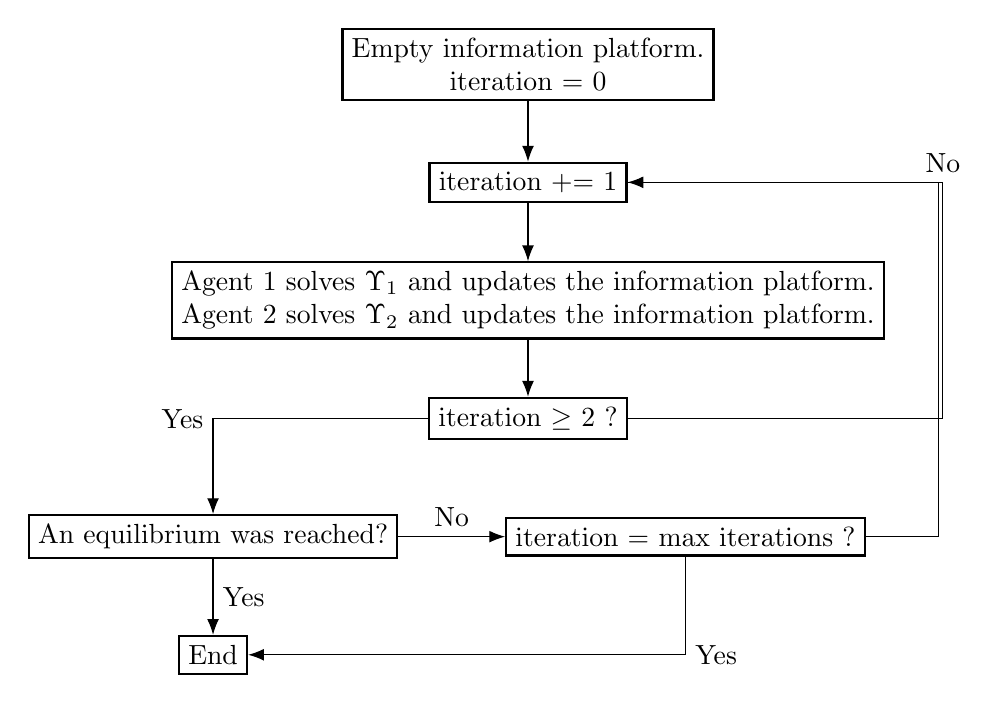
\begin{tikzpicture}
\begin{scope}[every node/.style={rectangle,draw,thick}]
	\node[align = center] (init) at (0,0)  {Empty information platform.\\
	iteration = 0};
	\node (iteration) at (0,-1.5){iteration += 1};
	\node[align =left] (main) at (0,-3) {Agent 1 solves $\Upsilon_1$  and updates the information platform.\\
	Agent 2 solves $\Upsilon_2$  and updates the information platform.};
	\node (itquestion) at (0,-4.5) {iteration $\geq$ 2 ?};

	\node (equiquestion) at (-4,-6) {An equilibrium was reached?};

	\node (maxit) at (2,-6) {iteration = max iterations ?};

	\node (End) at (-4,-7.5) {End};
\end{scope}

\begin{scope}
	\draw[-{Latex[length=2mm]}] (init) edge (iteration);
	\draw[-{Latex[length=2mm]}] (iteration) edge (main);
	\draw[-{Latex[length=2mm]}] (main) edge (itquestion);
	\draw[-{Latex[length=2mm]}] (itquestion.east)  -- ++(4cm,0) |- node[above] {No}
	 (iteration.east);
	\draw[-{Latex[length=2mm]}] (itquestion.west) -| node[left] {Yes} (equiquestion);
	\draw[-{Latex[length=2mm]}] (equiquestion)  edge node[above] {No} (maxit);
	\draw[-{Latex[length=2mm]}] (equiquestion) edge node[right] {Yes} (End);
	\draw[-{Latex[length=2mm]}] (maxit.south) |- node[right] {Yes} (End);
	\draw[-] (maxit.east)  -- ++(0.92cm,0) |- (iteration.east);
\end{scope}
\end{tikzpicture}
\end{adjustbox}
\end{figure}

\end{frame}

\section{Computationally results}

\begin{frame}{Instances}
	\begin{itemize}
		\setlength\itemsep{1em}
		\item Instances with 2 and 5 agents.
		\item Graph with 7 nodes.
		\item Complete graph for all the agents.
		\item All the parameters selected from uniform distributions.
		\item Instances with edges with LOW or HIGH capacity.
	\end{itemize}
\end{frame}

\begin{frame}{Results: Instances with 2 agents}
\only<1>{
\begin{figure}
\begin{adjustbox}{width=\textwidth, totalheight=\textheight-2\baselineskip,keepaspectratio}
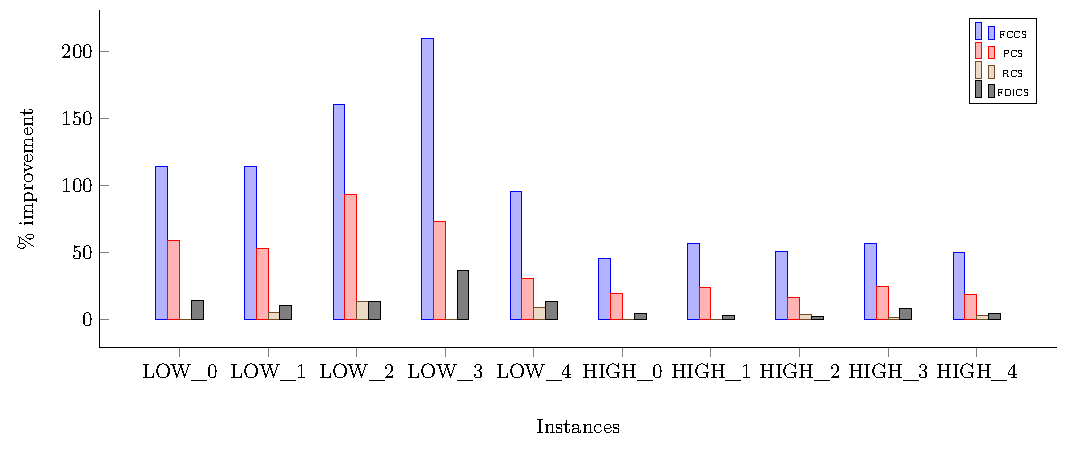
\includegraphics[scale=1]{graphs.pdf}
\end{adjustbox}
\end{figure}
}
\only<2>{
\begin{figure}
\begin{adjustbox}{width=\textwidth, totalheight=\textheight-2\baselineskip,keepaspectratio}
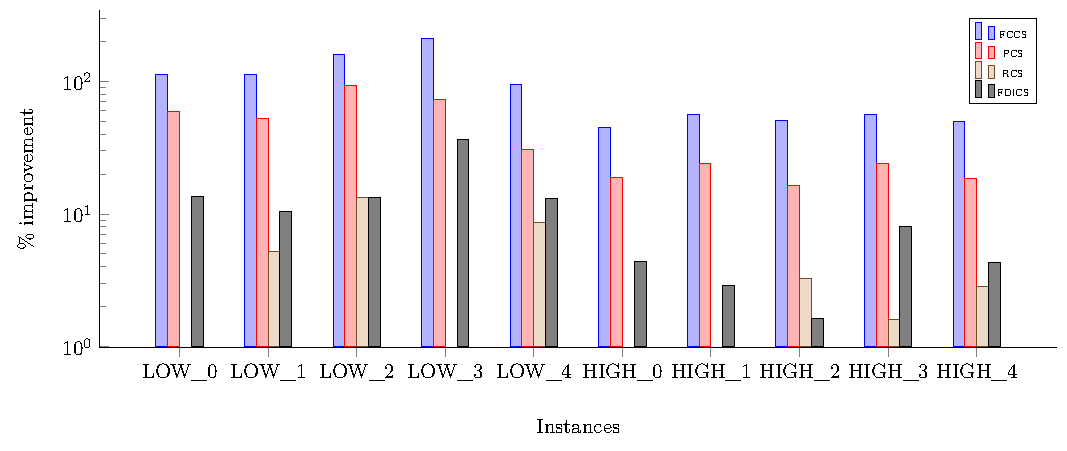
\includegraphics[scale=1]{graphs_log.pdf}
\end{adjustbox}
\end{figure}
}
\end{frame}

\begin{frame}{Results: Analysis of order relevance in FDICS}

\begin{table}[ht!]
\centering
\begin{adjustbox}{max width=\textwidth}
\begin{tabular}{lrrrrrr}
\toprule
{} & \multicolumn{2}{c}{Total payoffs} & \multirow{2}{*}{\% Dif.} & \multicolumn{2}{c}{Nº iterations} & \multirow{2}{*}{\ Dif.} \\
{} &  Order:1-2 &  Order:2-1 &       &  Order:1-2 &  Order:2-1 & \\
\midrule
2\_low\_0  &           25.0 &           25.0 &  0.00 &        4.0 &        3.0 &     1.0 \\
2\_low\_1  &           21.0 &           21.0 &  0.00 &        3.0 &        3.0 &     0.0 \\
2\_low\_2  &           17.0 &           17.0 &  0.00 &        3.0 &        3.0 &     0.0 \\
2\_low\_3  &           15.0 &           15.0 &  0.00 &        4.0 &        4.0 &     0.0 \\
2\_low\_4  &           27.0 &           26.0 &  3.70 &        3.0 &        3.0 &     0.0 \\
2\_high\_0 &           73.0 &           72.0 &  1.37 &        3.0 &        3.0 &     0.0 \\
2\_high\_1 &           70.0 &           69.0 &  1.49 &        3.0 &        3.0 &     0.0 \\
2\_high\_2 &           65.0 &           63.0 &  3.08 &        3.0 &        3.0 &     0.0 \\
2\_high\_3 &           68.0 &           67.0 &  1.47 &        4.0 &        4.0 &     0.0 \\
2\_high\_4 &           74.0 &           73.0 &  1.35 &        3.0 &        3.0 &     0.0 \\
\bottomrule
\end{tabular}
\end{adjustbox}
\end{table}
\end{frame}


\section{Conclusions}

\begin{frame}{\secname}
\begin{itemize}
\setlength\itemsep{1em}
\item<1-> In terms of solution quality: FCCS > PCS > \alert{FDICS > RCS}.
\item<2-> Relevance of amount of information shared and decision power allocation.
\item<3-> Extension of FDICS to more agents might be interesting.
\end{itemize}
\end{frame}

\metroset{numbering=none}
\begin{frame}[noframenumbering]
\begin{center}
  \Large{Thank you for the attention.}
\end{center}
\end{frame}

\end{document}